\documentclass[10pt]{article}
\usepackage{graphicx}
\graphicspath{ {images/} }

\begin{document}

\title{Homework 1 - Sets}
\author{Michael Gould\\ 
CS 506 - Online Foundations of CS}
 
\maketitle

1. Let A $= \{1,3,5\}$ and B $= \{2,3,4\}$.  Determine each of the following \\sets.

$A \cup B = \{1,2,3,4,5\}$

$A \cap B = \{3\}$

$A - B = \{1,5\}$

$B - A = \{2,4\}$

$(A \cup B) - (A \cap B ) = \{1,2,4,5\}$

$(A - B) \cup (B - A) = \{1,2,4,5\}$\\


2. Prove the following set-equality, first by Venn Diagram, and then by algebraic method.

$$(A \cup B) \cap \overline{(A \cap B )}  = (A \cap \overline{B}) \cup (\overline{A} \cap B)$$

The algebraic proof uses set algebraic manipulations to prove the equality, by using valid algebraic rules already proven.  The basic rules listed in the table below are assumed to have been proven, and thus are valid rules to use.

Venn Diagram:\\

Left Side:

$A \cap B$\\
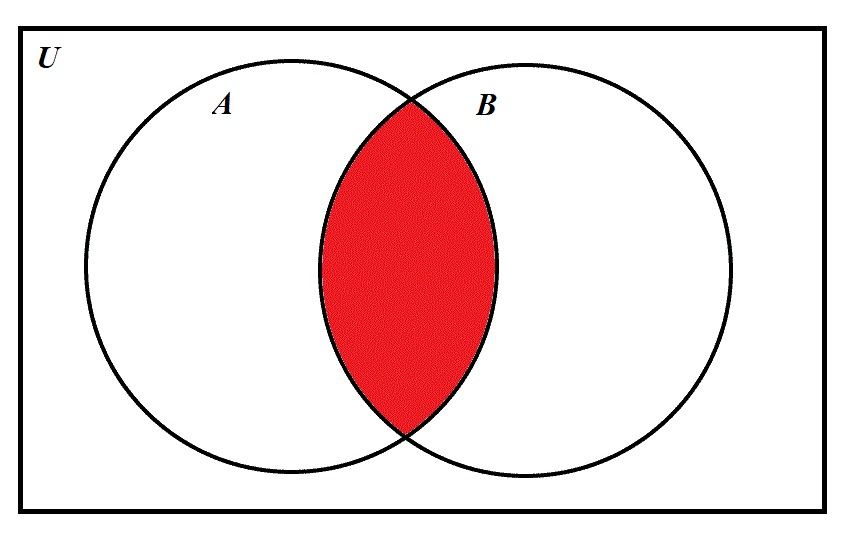
\includegraphics[scale=0.3]{1}

$\overline{A \cap B}$\\
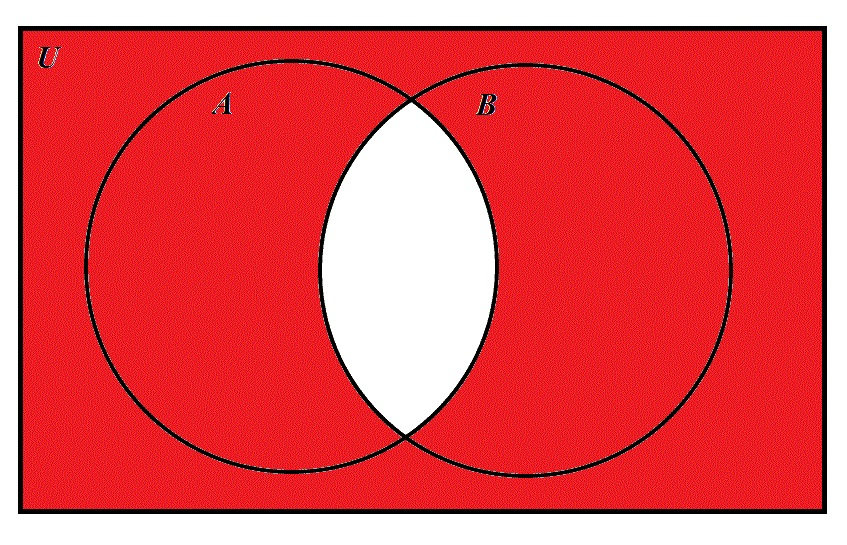
\includegraphics[scale=0.3]{2}

$A \cup B$\\
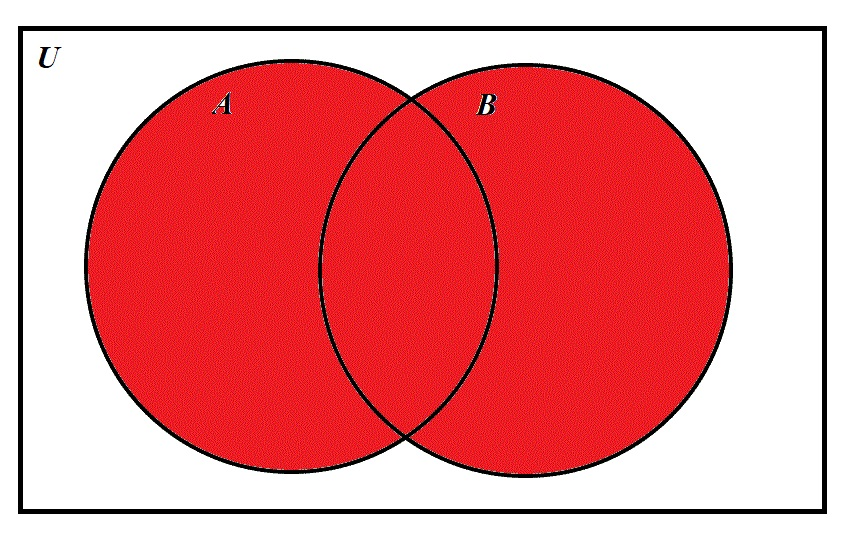
\includegraphics[scale=0.3]{3}

$(A \cup B) \cup \overline{(A \cap B)}$\\
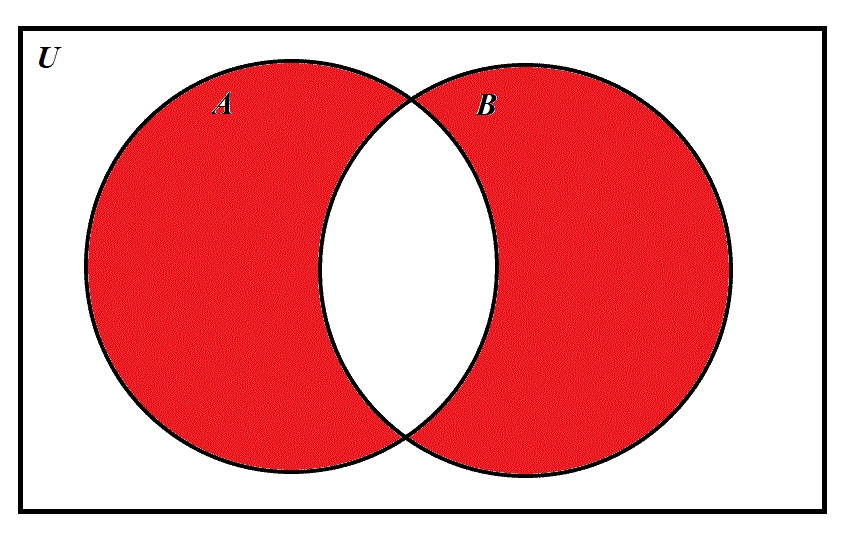
\includegraphics[scale=0.3]{4}

Right Side:

$\overline{B}$\\
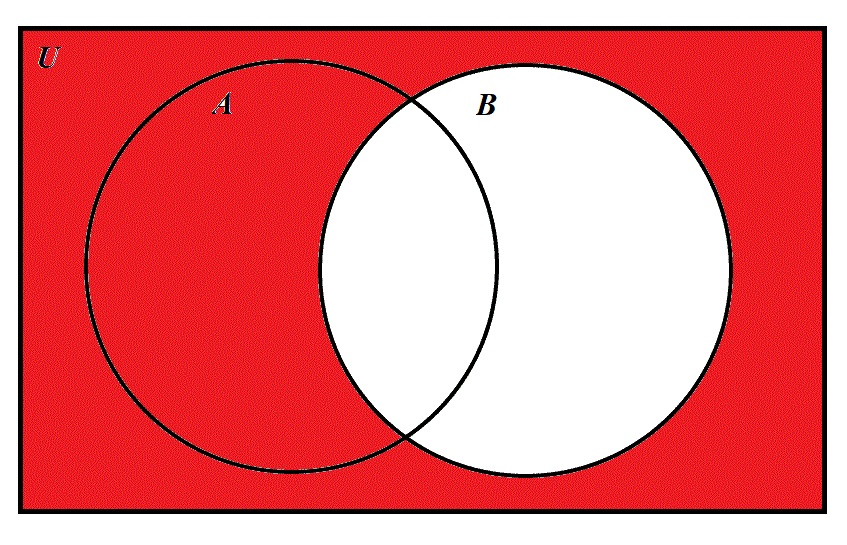
\includegraphics[scale=0.3]{5}

$A \cap \overline{B}$\\
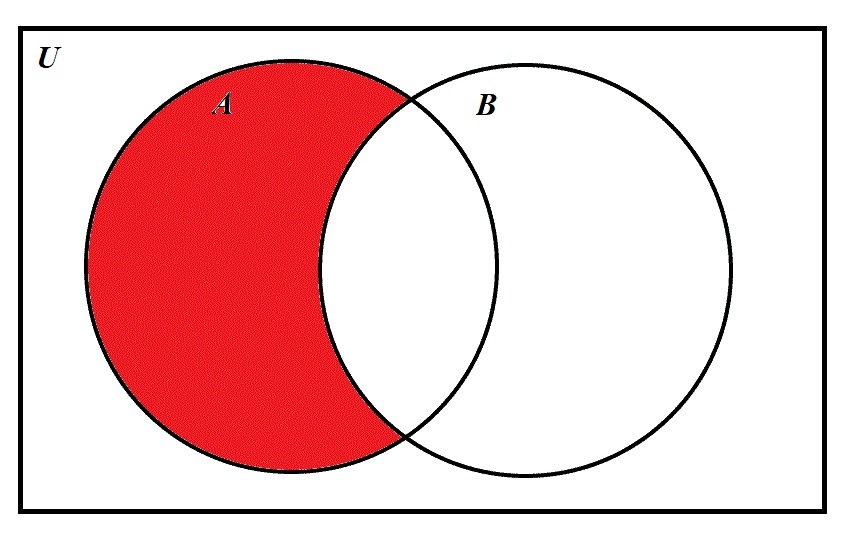
\includegraphics[scale=0.3]{6}

$\overline{A}$\\
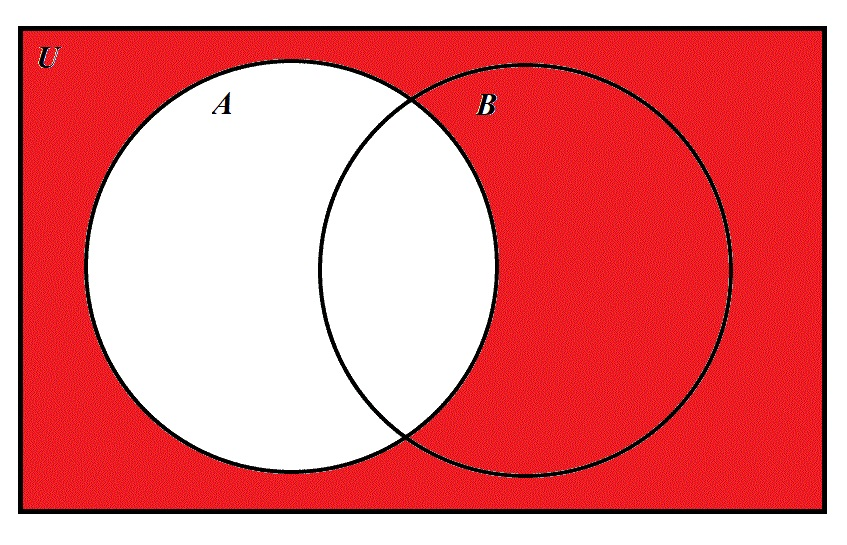
\includegraphics[scale=0.3]{7}

$\overline{A} \cap B$\\
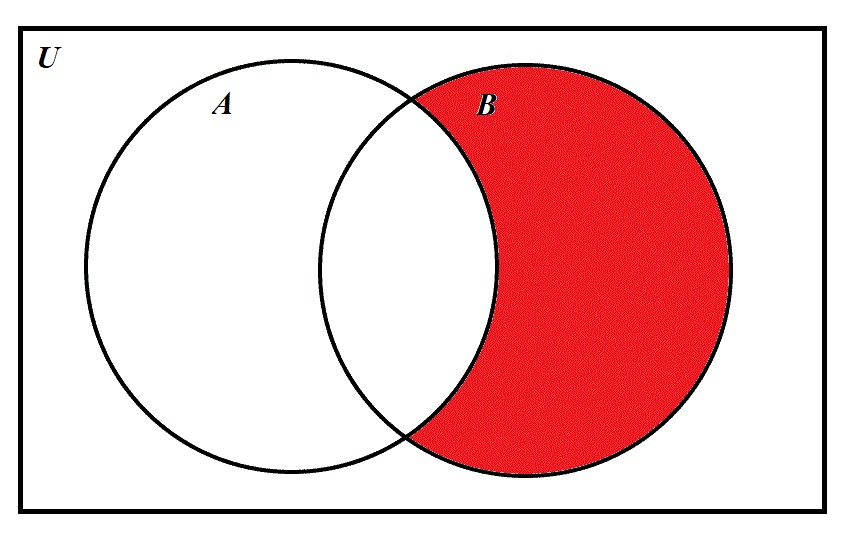
\includegraphics[scale=0.3]{8}

$(A \cup B) \cup \overline{(A \cap B)}$\\
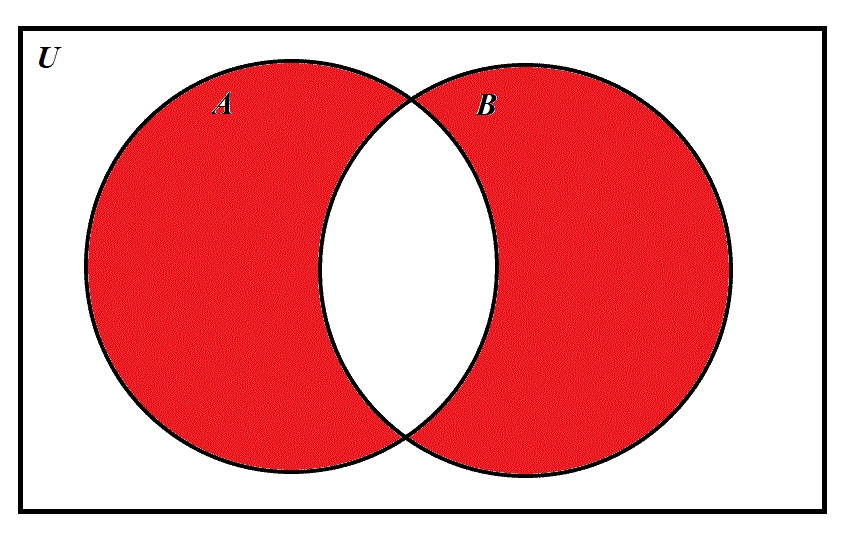
\includegraphics[scale=0.3]{4}

Algebraic Proof:

$$(A \cup B) \cap \overline{(A \cap B )}  = (A \cap \overline{B}) \cup (\overline{A} \cap B)$$

De Morgan's Law:
$$(A \cap B) \cup (\overline{A} \cup \overline{B}) = (A \cap \overline{B}) \cup (\overline{A} \cap B)$$

Distributive Law
$$((A \cup B) \cap \overline{A}) \cup ((A \cup B) \cap \overline{B}) = (A \cap \overline{B}) \cup (\overline{A} \cap B)$$

Distributive Law
$$((A \cap \overline{A}) \cup (B \cap \overline{A})) \cup ((A \cup B) \cap \overline{B}) = (A \cap \overline{B}) \cup (\overline{A} \cap B)$$

Distributive Law
$$((A \cap \overline{A}) \cup (B \cap \overline{A})) \cup ((A \cap \overline{B}) \cup (B \cap \overline{B})) = (A \cap \overline{B}) \cup (\overline{A} \cap B)$$

Complement Law
$$((U) \cup (B \cap \overline{A})) \cup ((A \cap B) \cup (B \cup \overline{B}) = (A \cap \overline{B}) \cup (\overline{A} \cap B)$$

Complement Law
$$((U) \cup (B \cap \overline{A})) \cup ((A \cap B) \cup (U) = (A \cap \overline{B}) \cup (\overline{A} \cap B)$$

Identity Law
$$(B \cap \overline{A}) \cup ((A \cap B) \cup (U) = (A \cap \overline{B}) \cup (\overline{A} \cap B)$$

Identity Law
$$(B \cap \overline{A}) \cup (A \cap B) = (A \cap \overline{B}) \cup (\overline{A} \cap B)$$

Commutative Law  
$$(A \cap \overline{B}) \cup (\overline{A} \cap B) = (A \cap \overline{B}) \cup (\overline{A} \cap B)$$

3. Prove each of the following set equalities by algebraic method.  In the proofs, you may use the basic rules listed in the table above.\\

(a) Combination Rule:
$$(A \cap B) \cup (A \cap \overline{B}) = A$$

Distributive Law
$$A \cap (B \cup \overline{B}) = A$$

Complement Law
$$A \cap (U) = A$$

Identity Law
$$A = A$$\\

(b) Absorption Rule:
$$ A \cup (A \cap B) = A$$

Identity Law
$$(A \cup U) \cup (A \cap B) = A$$

Distributiive Law
$$A \cap (U \cup B) = A$$

Commutative Law
$$A \cap(B \cup U) = A$$

Bound Law
$$A \cup U = A$$

Identity Law
$$A = A$$

Hint: If you start by distributive law, you will not find it useful.  Instead, first replace the leftmost $A$ by $A \cup U$ and then apply the distributiive law.  Alternatively, you may find the above "combination rule" useful.\\

(c)
$$A \cup (\overline{A} \cap B) = A \cup B$$

Distributive Law
$$(A \cup \overline{A}) \cap (A \cup B) = A \cup B$$

Complement Law
$$U \cap (A\cup B) = A \cup B$$

Commutative Law
$$(A\cup B) \cap U = A \cup B$$

Identity Law
$$A \cup B = A \cup B$$\\

(d)
$$(A \cap \overline{B}) \cup (A \cap B) \cup (\overline{A} \cap B) = A \cup B$$

Distributive Law
$$A \cap (B \cup \overline{B}) \cup (\overline{A} \cap B) = A \cup B$$

Complement Law
$$A \cap U \cup (\overline{A} \cap B) = A \cup B$$

Identity Law
$$A \cup (\overline{A} \cap B) = A \cup B$$

Distributive Law
$$(A \cup \overline{A}) \cap (A \cup B) = A \cup B$$

Complement Law
$$U \cap (A \cup B) = A \cup B$$

Identity Law
$$A\cup B = A \cup B$$

4. (a) Use Venn Diagrams to prove each of the following.

i.
$$A - B = A \cap \overline{B}$$

Left Side:

$A$\\
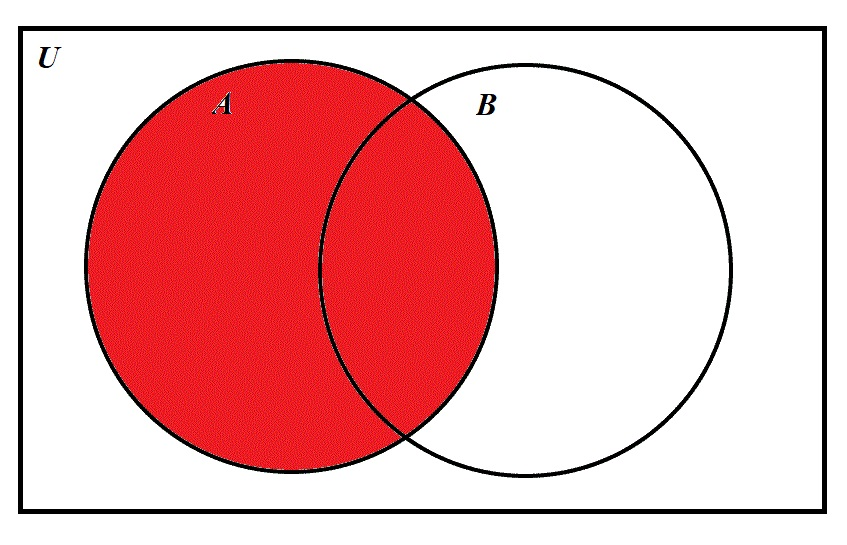
\includegraphics[scale=0.3]{9}

$B$\\
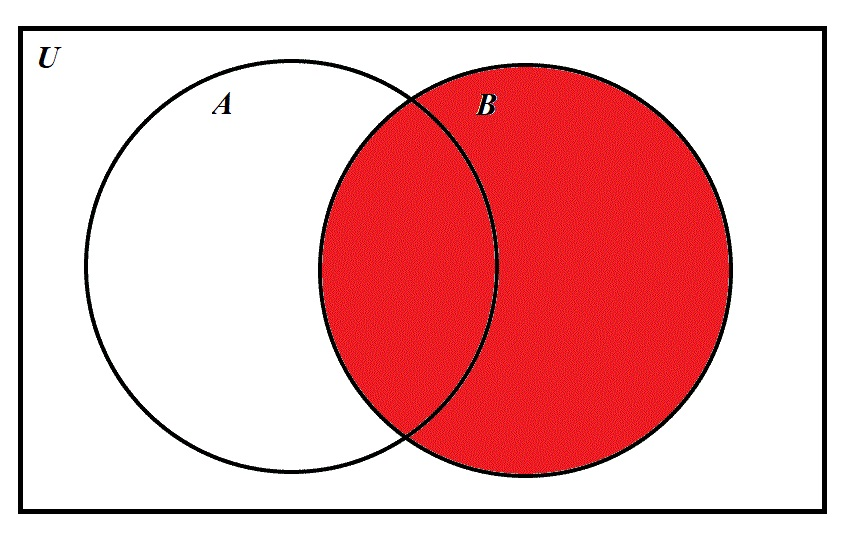
\includegraphics[scale=0.3]{10}

$A - B$\\
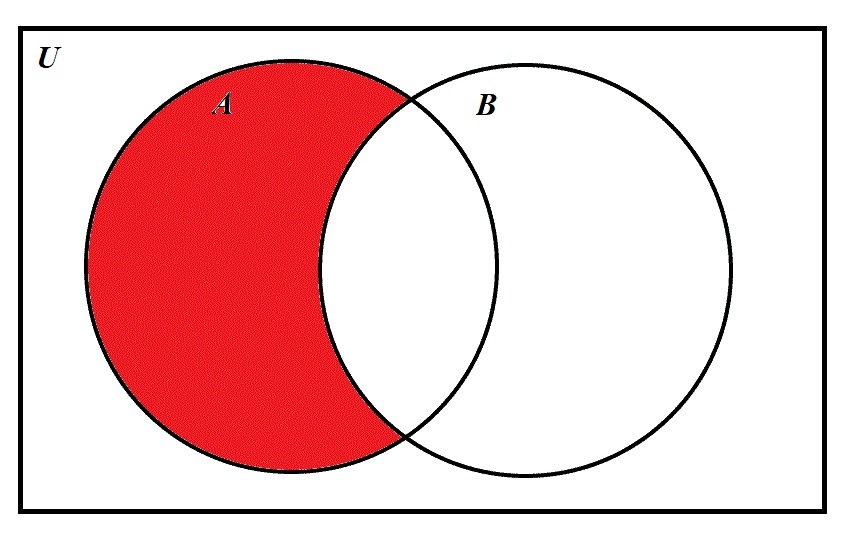
\includegraphics[scale=0.3]{11}

Right Side:

$A$\\
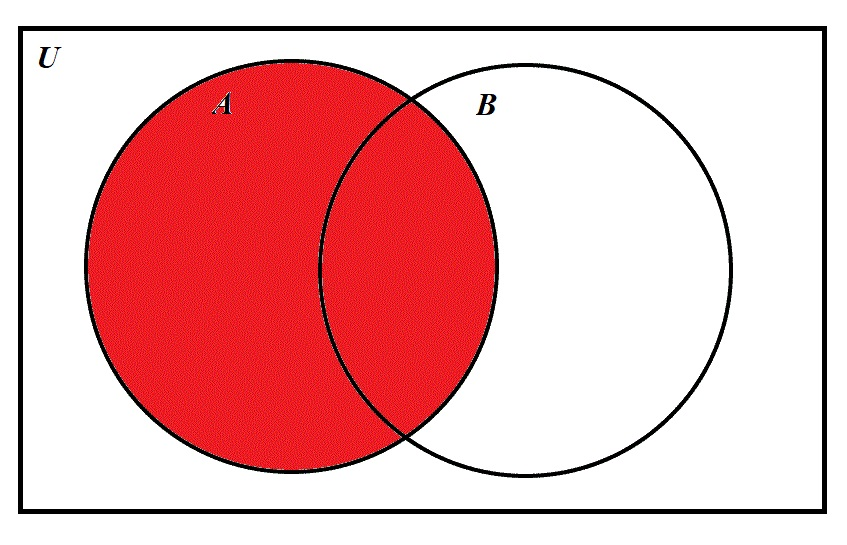
\includegraphics[scale=0.3]{9}

$\overline{B}$\\
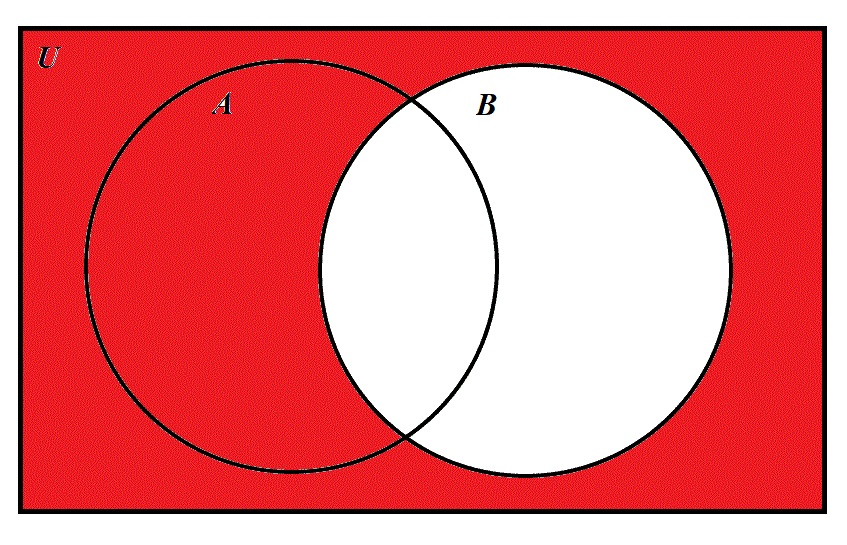
\includegraphics[scale=0.3]{5}

$A \cap \overline{B}$\\
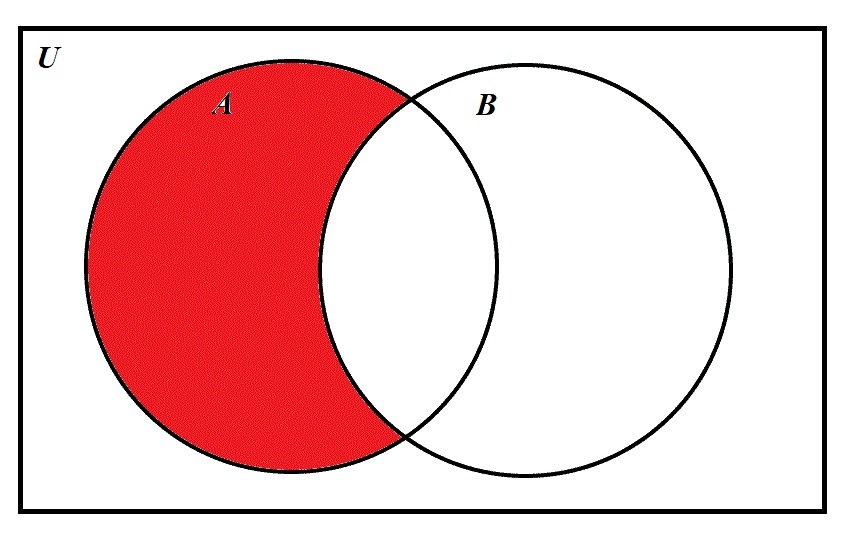
\includegraphics[scale=0.3]{11}

ii.
$$(A - B) - C = A \cap \overline{B} \cap \overline{C}$$

Left Side::

$A$\\
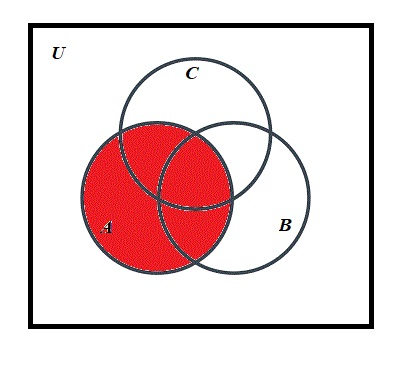
\includegraphics[scale=0.55]{12}

$B$\\
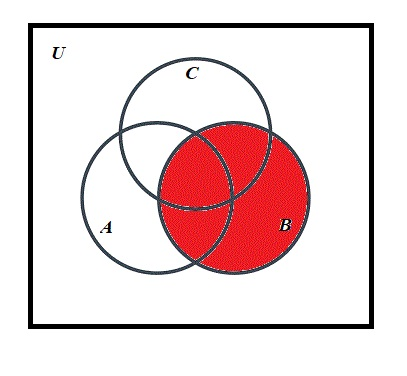
\includegraphics[scale=0.55]{13}

$A - B$\\
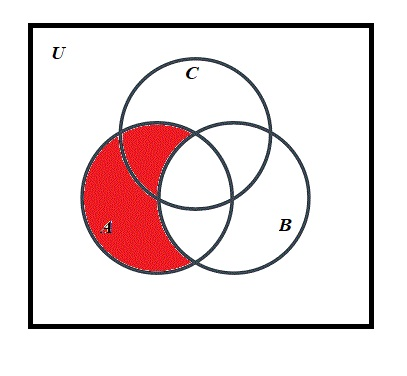
\includegraphics[scale=0.55]{15}

$C$\\
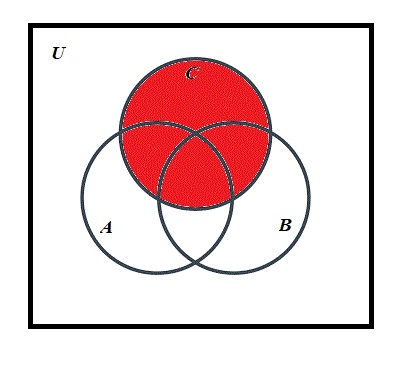
\includegraphics[scale=0.55]{14}

$(A - B) - C$\\
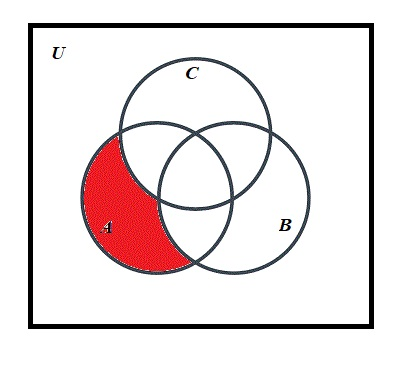
\includegraphics[scale=0.55]{16}

Right Side:

$A$\\
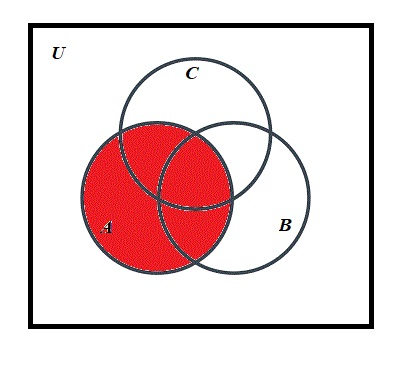
\includegraphics[scale=0.55]{12}

$\overline{B}$\\
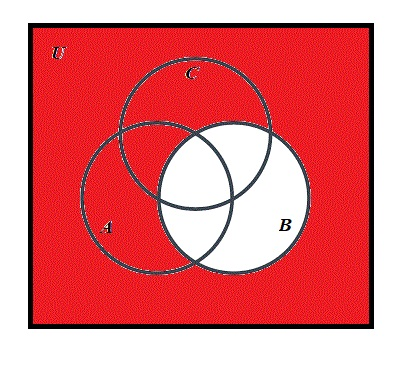
\includegraphics[scale=0.55]{17}

$A \cap \overline{B}$\\
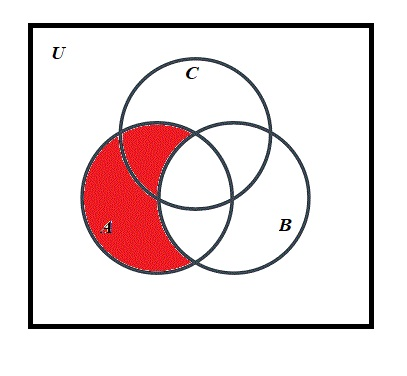
\includegraphics[scale=0.55]{18}

$\overline{C}$\\
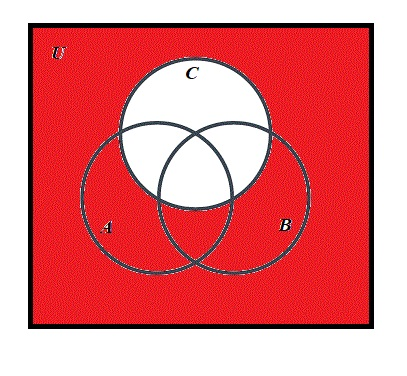
\includegraphics[scale=0.55]{19}

$A \cap \overline{B} \cap \overline{C}$\\
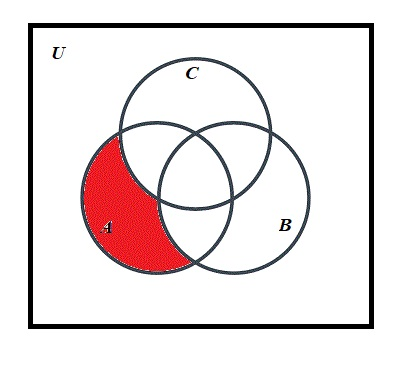
\includegraphics[scale=0.55]{20}

(b)Use the algebraic method to prove each of the following set qualities.
Hint: The rules stated in the above table, such as Associate law, DeMorgan law and Distributitve law, apply only to intersection and union operations.  They do NOT apply to other operations such as set difference.  To deal with set difference, it is helpful to first replace set-difference with the cooresponding rule that uses set complement.\\

i.
$$A - (B - C) = (A \cap \overline{B}) \cup (A \cap C)$$

Cooresponding Set-difference Rule
$$A - (B \cap \overline{C}) = (A \cap \overline{B}) \cup (A \cap C)$$

Cooresponding Set-difference Rule
$$A \cap \overline{(B \cap \overline{C})} = (A \cap \overline{B}) \cup (A \cap C)$$

DeMorgan's Law
$$A \cap (\overline{B} \cup \overline{\overline{C}}) = (A \cap \overline{B}) \cup (A \cap C)$$

Complement Law
$$A \cap (\overline{B} \cup C) = (A \cap \overline{B}) \cup (A \cap C)$$

Distributive Law
$$(A \cap \overline{B}) \cup (A \cap C) = (A \cap \overline{B}) \cup (A \cap C)$$\\

ii. 
$$\overline{(A - B)} = \overline{A} \cup B$$

Cooresponding Set-difference Rule
$$\overline{(A \cap \overline{B})} = \overline{A} \cup B$$

DeMorgan's Law
$$\overline{A} \cup \overline{\overline{B}} = \overline{A} \cup B$$

Complement Law
$$\overline{A} \cup B = \overline{A} \cup B$$\\

iii.
$$A \cap \overline{(A \cap B)} = A \cap \overline {B}$$

Demorgan's Law
$$A \cap (\overline{A} \cup \overline{B}) = A \cap \overline {B}$$

Distributive Law
$$(A \cap \overline{A}) \cup (A \cap \overline{B}) = A \cap \overline {B}$$

Complement Law
$$\emptyset \cup (A \cap \overline{B}) = A \cap \overline {B}$$

Identity Law
$$A \cap \overline {B} = A \cap \overline {B}$$\\

5. Prove each of the following set equalities both by Venn Diagram and by algebraic method.\\

Venn Diagram:

(a)
$$A - (B \cap C) = (A - B) \cup (A - C)$$

Left Side:

$B \cap C$\\
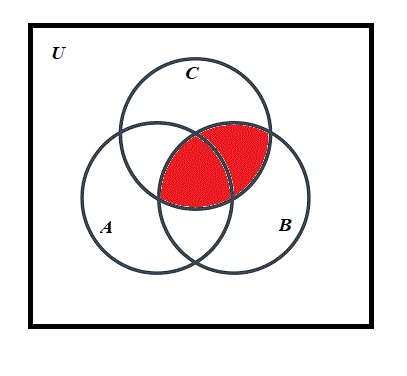
\includegraphics[scale=0.55]{21}

$A$\\
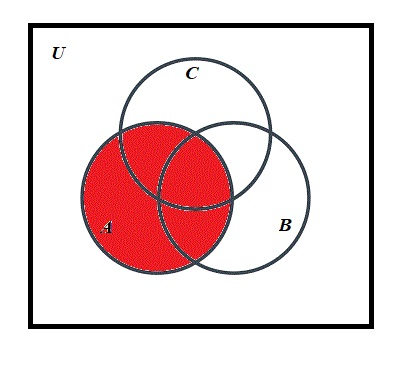
\includegraphics[scale=0.55]{12}

$A - (B \cap C)$\\
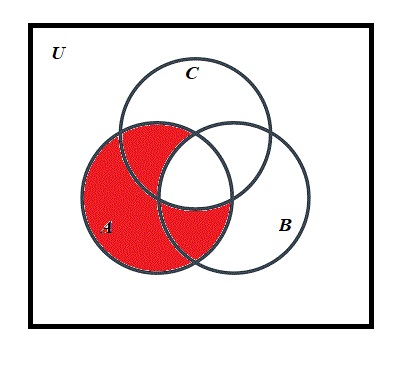
\includegraphics[scale=0.55]{22}

Right Side:

$A - B$\\
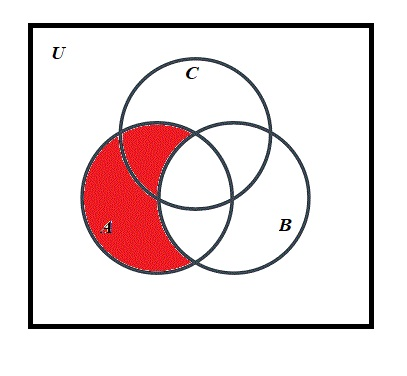
\includegraphics[scale=0.55]{18}

$A - C$\\
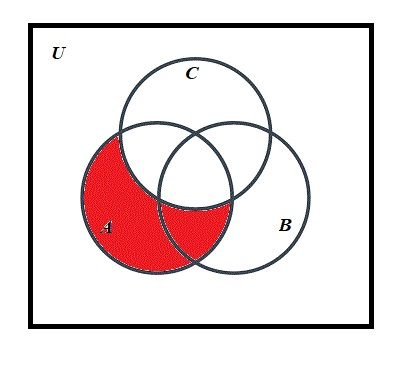
\includegraphics[scale=0.55]{23}

$(A - B) \cup (A - C)$\\
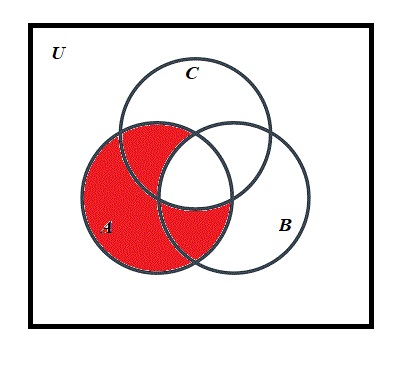
\includegraphics[scale=0.55]{22}

(b)
$$A - (B \cup C) = (A - B \cap (A - C)$$\\

Left Side:

$A$\\
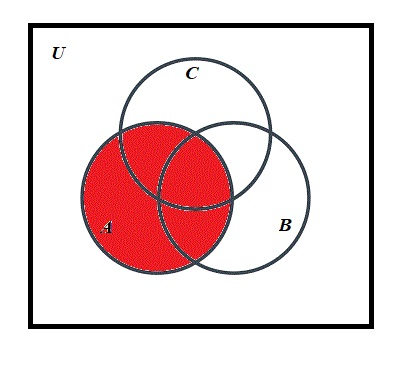
\includegraphics[scale=0.55]{12}

$B \cup C$\\
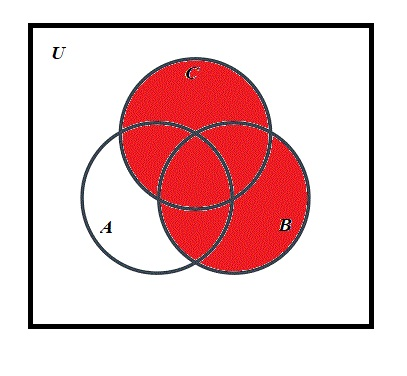
\includegraphics[scale=0.55]{24}

$A - (B \cup C)$\\
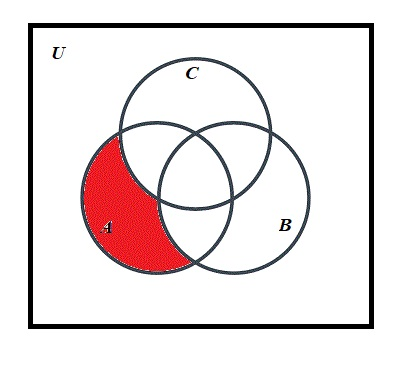
\includegraphics[scale=0.55]{25}

Right Side:

$A - B$\\
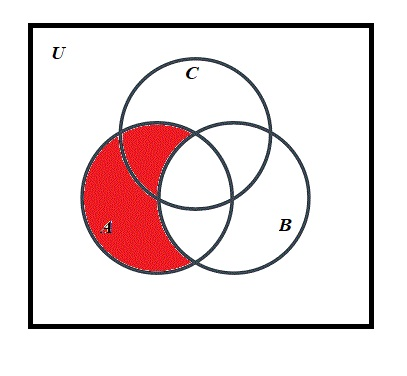
\includegraphics[scale=0.55]{18}

$A - C$\\
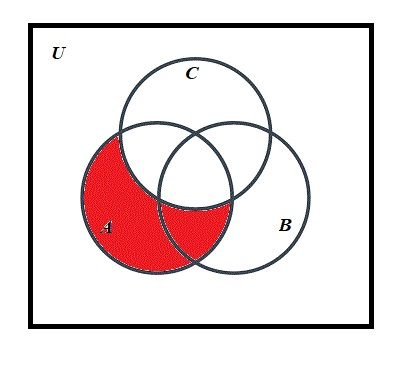
\includegraphics[scale=0.55]{23}

$(A - B) \cup (A - C)$\\
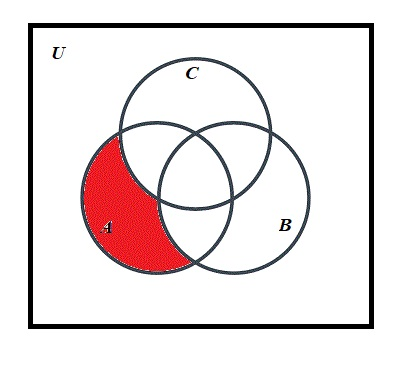
\includegraphics[scale=0.55]{25}

(c)
$$A \cap (B - C) = (A \cap B) -  C = (A \cap B) - (A \cap C)$$\\

Left Side:

$B - C$\\
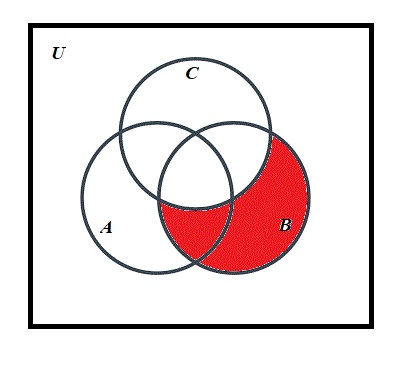
\includegraphics[scale=0.55]{26}

$A$\\
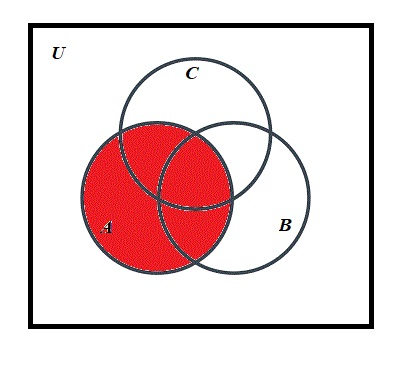
\includegraphics[scale=0.55]{12}

$A \cap (B - C)$\\
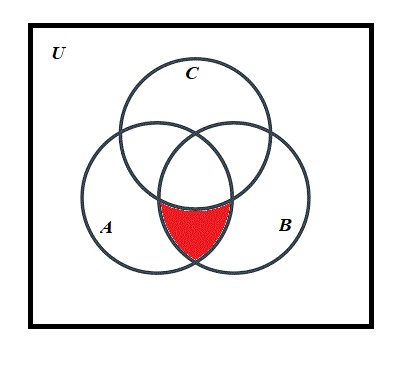
\includegraphics[scale=0.55]{27}

Middle:

$A \cap B$\\
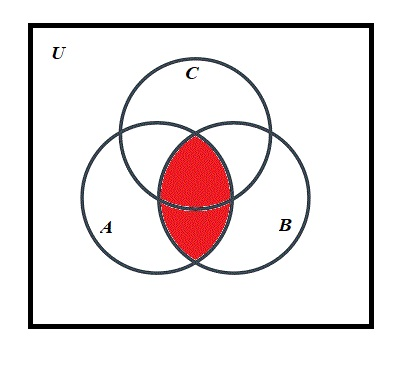
\includegraphics[scale=0.55]{28}

$C$\\
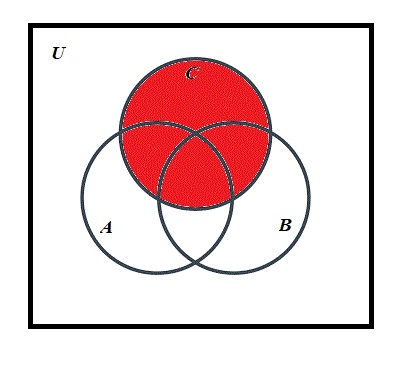
\includegraphics[scale=0.55]{14}

$(A \cap B) - C$\\
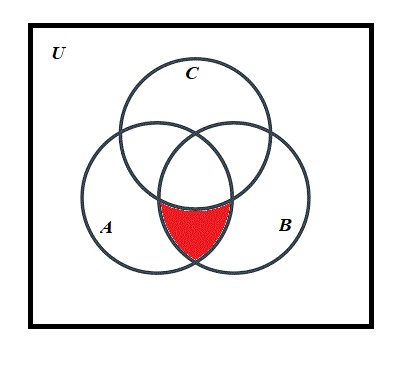
\includegraphics[scale=0.55]{27}

Right:

$A \cap B$\\
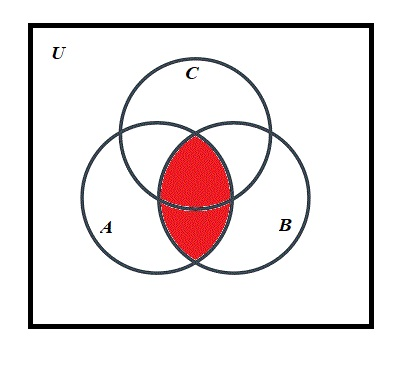
\includegraphics[scale=0.55]{28}

$A \cap C$\\
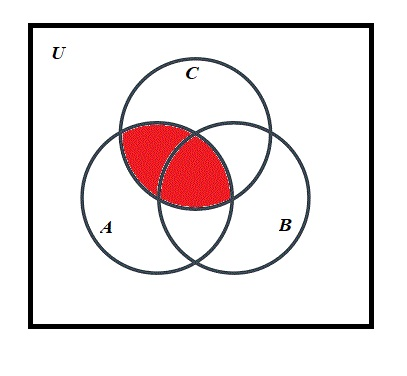
\includegraphics[scale=0.55]{29}

$(A \cap B) - (A \cap C)$\\
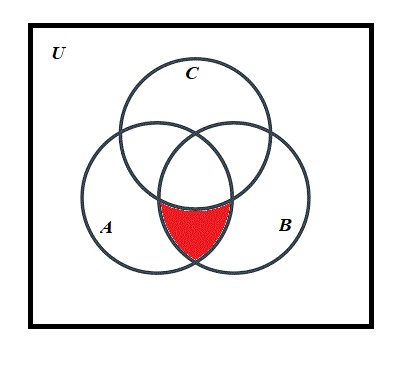
\includegraphics[scale=0.55]{27}

Hint: To prove the last form, use the equality $A \cap \overline{C} = A \cap (\overline{A} \cap \overline{C})$.\\

(d)
$$A \cup (B - C) = (A \cup B) \cap (A \cup \overline{C}) = (A \cup B) - (\overline{A} \cap C)$$\\

Left Side:

$B - C$\\
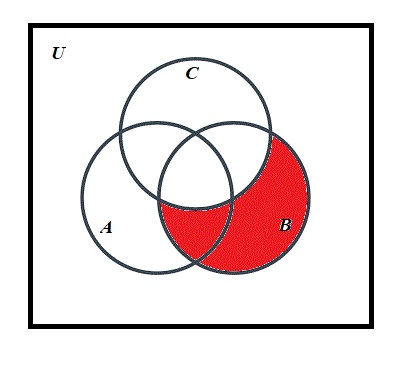
\includegraphics[scale=0.55]{26}

$A$\\
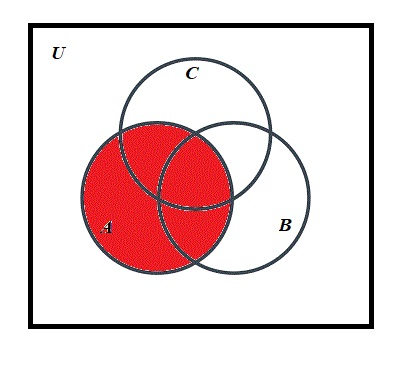
\includegraphics[scale=0.55]{12}

$A \cup (B - C)$\\
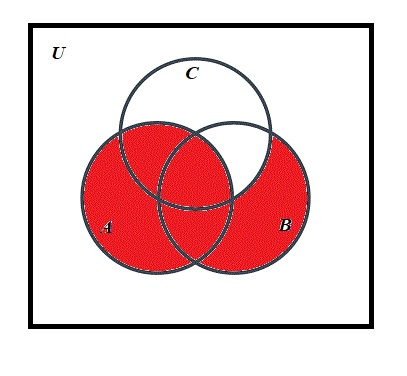
\includegraphics[scale=0.55]{30}

Middle:

$\overline{C}$\\
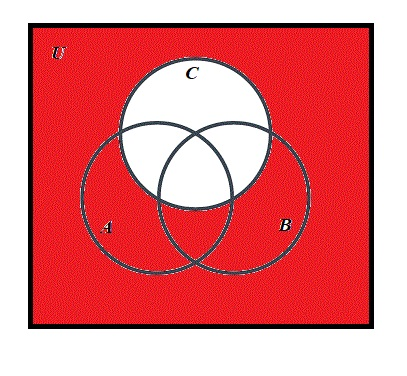
\includegraphics[scale=0.55]{19}

$A \cup \overline{C}$\\
\includegraphics[scale=0.55]{31}

$A \cup B$\\
\includegraphics[scale=0.55]{32}

$(A \cup B) \cap (A \cup \overline{C})$\\
\includegraphics[scale=0.55]{33}

Right Side:

$\overline{A}$\\
\includegraphics[scale=0.55]{34}

$\overline{A} \cap C$\\
\includegraphics[scale=0.55]{35}

$A \cup B$\\
\includegraphics[scale=0.55]{32}

$(A \cup B) - (\overline{A} \cap C)$\\
\includegraphics[scale=0.55]{33}

Algebraic Proof:

(a)
$$A - (B \cap C) = (A - B) \cup (A - C)$$

Set Difference Rule
$$A \cap \overline{(B \cap C)} = (A - B) \cup (A - C)$$

Set Difference Rule
$$A \cap \overline{(B \cap C)} = (A \cap \overline{B}) \cup (A - C)$$

Set Difference Rule
$$A \cap \overline{(B \cap C)} = (A \cap \overline{B}) \cup (A \cap \overline{C})$$

DeMorgan's Law
$$A \cap (\overline{B} \cup \overline{C}) = (A \cap \overline{B}) \cup (A \cap \overline{C})$$

Distributive Law
$$(A \cap \overline{B}) \cup (A \cap \overline{C}) = (A \cap \overline{B}) \cup (A \cap \overline{C})$$\\

(b)
$$A - (B \cup C) = (A - B) \cap (A - C)$$

Set Difference Rule
$$A \cap \overline{(B \cup C)} = (A - B) \cap (A - C)$$

Set Difference Rule
$$A \cap \overline{(B \cup C)} = (A \cap \overline{B}) \cap (A - C)$$

Set Difference Rule
$$A \cap \overline{(B \cup C)} = (A \cap \overline{B}) \cap (A \cap \overline{C})$$

DeMorgan's Law
$$A \cap (\overline{B} \cap \overline{C}) = (A \cap \overline{B}) \cap (A \cap \overline{C})$$

Distributive Law
$$(A \cap \overline{B}) \cap (A \cap \overline{C}) = (A \cap \overline{B}) \cap (A \cap \overline{C})$$\\

(c)
$$A \cap (B - C) = (A \cap B) -  C = (A \cap B) - (A \cap C)$$

Set Difference Rule
$$A \cap (B \cap \overline{C}) = (A \cap B) - C = (A \cap B) - (A \cap C)$$

Set Difference Rule
$$A \cap (B \cap \overline{C}) = (A \cap B) \cap \overline{C} = (A \cap B) - (A \cap C)$$

Set Difference Rule
$$A \cap (B \cap \overline{C}) = (A \cap B) \cap \overline{C} = (A \cap B) \cap \overline{(A \cap C)}$$

Associative Rule
$$A \cap (B \cap \overline{C}) = A \cap (B \cap \overline{C}) = (A \cap B) \cap \overline{(A \cap C)}$$

DeMorgan's Law
$$A \cap (B \cap \overline{C}) = A \cap (B \cap \overline{C}) = (A \cap B) \cap (\overline{A} \cup \overline{C})$$

Earlier Proven Qualities (Refer to 3c and hint equation)
$$A \cap (B \cap \overline{C}) = A \cap (B \cap \overline{C}) = (A \cap (\overline{A} \cup B)) \cap (A \cap (\overline{A} \cup \overline{C}))$$

Distributive Law
$$A \cap (B \cap \overline{C}) = A \cap (B \cap \overline{C}) = (A \cap \overline{A}) \cup (A \cap B) \cap (A \cap (\overline{A} \cup \overline{C}))$$

Distrubitive Law
$$A \cap (B \cap \overline{C}) = A \cap (B \cap \overline{C}) = (A \cap \overline{A}) \cup (A \cap B) \cap (A \cap \overline{A}) \cup (A \cap \overline{C})$$

Complement Law
$$A \cap (B \cap \overline{C}) = A \cap (B \cap \overline{C}) = \emptyset \cup (A \cap B) \cap (A \cap \overline{A}) \cup (A \cap \overline{C})$$

Complement Law
$$A \cap (B \cap \overline{C}) = A \cap (B \cap \overline{C}) = \emptyset \cup (A \cap B) \cap \emptyset \cup (A \cap \overline{C})$$

Identity Law
$$A \cap (B \cap \overline{C}) = A \cap (B \cap \overline{C}) =  (A \cap B) \cap \emptyset \cup (A \cap \overline{C})$$

Identity Law
$$A \cap (B \cap \overline{C}) = A \cap (B \cap \overline{C}) = (A \cap B) \cap (A \cap \overline{C})$$

Distributive Law
$$A \cap (B \cap \overline{C}) = A \cap (B \cap \overline{C}) = (A \cap (B \cap \overline{C})$$

Hint: To prove the last form, use the equality $A \cap \overline{C} = A \cap (\overline{A} \cap \overline{C})$.\\

(d)
$$A \cup (B - C) = (A \cup B) \cap (A \cup \overline{C}) = (A \cup B) - (\overline{A} \cap C)$$

Set Difference Rule
$$A \cup (B \cap \overline{C}) = (A \cup B) \cap (A \cup \overline{C}) = (A \cup B) - (\overline{A} \cap C)$$

Set Difference Rule
$$A \cup (B \cap \overline{C}) = (A \cup B) \cap (A \cup \overline{C}) = (A \cup B) \cap \overline{(\overline{A} \cap C)}$$

Distributive Law
$$A \cup (B \cap \overline{C}) = A \cap ( B \cup \overline{C}) = (A \cup B) \cap \overline{(\overline{A} \cap C)}$$

DeMorgan's Law
$$A \cup (B \cap \overline{C}) = A \cap ( B \cup \overline{C}) = (A \cup B) \cap (\overline{\overline{A}} \cup \overline{C})$$

Complement Law
$$A \cup (B \cap \overline{C}) = A \cap ( B \cup \overline{C}) = (A \cup B) \cap (A \cup \overline{C})$$

Distributive Law
$$A \cup (B \cap \overline{C}) = A \cap ( B \cup \overline{C}) = A \cap ( B \cup \overline{C})$$
\end{document}
